\documentclass[a4paper, 12pt]{article}

%\usepackage[margin=1in]{geometry}
\usepackage{graphicx}
\usepackage{float}
\usepackage{amsmath}
\usepackage{times}
\usepackage{parskip}
\usepackage[hidelinks]{hyperref}
\usepackage{titlesec}
\setcounter{secnumdepth}{4}
\setcounter{tocdepth}{4}
\titleformat{\paragraph}
{\normalfont\normalsize\bfseries}{\theparagraph}{1em}{}
\titlespacing*{\paragraph}
{0pt}{3.25ex plus 1ex minus .2ex}{1.5ex plus .2ex}

\usepackage{xurl}

\begin{document}

\begin{titlepage}

\begin{center}



\includegraphics[scale=0.6]{Images/UONLogo.png}

\vspace*{12pt}

School of Computer Science

University of Nottingham

Malaysia

\rule{\linewidth}{0.4pt}

\vspace{12pt}

{\Large Tree Segmentation Engine \& Toolkits for Oil Palm Plantation}

\vspace{12pt}

G52GRP Interim Group Report (Group L)

13 December 2022

Word Count: 4525

\rule{\linewidth}{0.4pt}

\vspace{12pt}

\textit{Members}

Tan Zhi Xuan 20305881

Wong Zhan Choon 20312555

Park Dong Kwan 20307405

Yeo Zen 20416394

Chelsea Khor Yen Wei 20305307

\vspace{12pt}

\textit{Supervised by}

Dr. Iman Yi Liao

\vspace{12pt}

\textit{Main Client}

Dr. Chen Zi Yan

Advanced Agriecological Research Sdn. Bhd. (AAR)

\end{center}

    
\end{titlepage}

\addcontentsline{toc}{section}{Abstract}
\begin{abstract}
    The world's largest producer of palm oil in Southeast Asia. \linebreak Since Malaysia significantly depends on palm oil as a key source of national income, effective management of oil palm plantations is crucial. Remote sensing tools like aerial LiDAR have been an aid for geographical mapping and remote monitoring of large terrains in crop management as it is time-consuming and requires more human resources when using conventional methods such as physically surveying oil palm land. Hence, LiDAR was used to scan the land, obtain the point cloud data and process the data by using the Tree Segmentation Engine that provides users with a comprehensive solution and tools. Ground Classifier provides a simple approach for users to perform complex pre-processing and classifying point cloud data. Height Normalizer was performed to process classified points and result in getting a flat terrain and reducing the impact of terrain on measurements taken above ground.

Next, Canopy Height Model (CHM) Generator and Smoother were introduced to generate a canopy height model from a derived surface based on normalized point cloud data. Generated CHM will be further post-processed to fill up the empty pixels from point cloud data. Moreover, Tree Tops Detector was applied to locate the individual tree and Tree Segmentation will segmentate out the individual tree after detecting the individual tree tops located on that scanned terrain area. During the Tree Segmentation process, each extracted individual tree will be allocated a unique ID and color for 3D visualization and allow users to view a specific tree by using ID. Each extracted individual tree will be filed into an individual LAS/LAZ file and users can choose the specific individual tree to generate a convex hull on the point cloud of the individual extracted tree allowing users to perform analysis-related tasks such as tree metrics measurement, detect diseases, etc.
\end{abstract}

%\section*{Abstract}




\newpage

\tableofcontents




\newpage

\section{Introduction}

\subsection{Client}

Advanced Agriecological Research Sdn. Bhd. (AAR) is one of the leading tropical plantation crop research centers in Malaysia. This company is a private research organization that looks at over 250,000 hectares of oil palm and rubber estates in Peninsular Malaysia, Sabah, Sarawak, and Liberia. It was founded in July 1986 to manage and direct research on tropical plantation crops as well as provide agronomic advisory services. It is committed to ensuring the advancement in the plantation crops research of Malaysia.

\subsection{Project Description}

\subsubsection{Project Scoping}

\paragraph{Problem Description}

Oil palm plantations are often large in acre area, with tonnes of oil palm trees grown on that terrain, making the earth and plant-science-related study or analysis a challenging task. Those tasks that require researchers to conduct in-depth analyses on individual vegetation will take a significant amount of time and human resources if traditional methodologies and approaches are used. Thus, the client discusses in depth his issues and concerns and he intends to develop software that can take advantage of technological advancements to assist them to speed up and simplify their data processing and analysis work.

\paragraph{Key objectives of the project}

The project's main goal is to assist the customer in developing a tree segmentation engine that provides comprehensive solutions and tools to assist him with data processing, tree segmentation tasks, and analysis work. Our team will develop software with an advanced tree segmentation pipeline built in that will lead the user through the tree segmentation processes of ground classification, height normalization, canopy height model (CHM) generator, and smoother, individual tree top identification, as well as tree segmentation. The software will also process the output of individual tree point cloud files by constructing a convex hull, making future analysis work easier.

\paragraph{Product Features}

The key features of our product will be the following:


\textbf{LAS/LAZ Point Cloud Renderer:} The user can load the LAS/LAZ file (point cloud data) into the software, and the application will interpret the file and build a high-resolution and high-quality 3D render view of the terrain in a point cloud format, allowing the user to easily analyze the point cloud data in a macro view. Furthermore, during point cloud data processing, this function will provide instant feedback to the user and assist the user in finding the ideal algorithm parameters for their data in a user-friendly manner.

\textbf{Ground Classifier:} The built-in ground classifier will help the user to process raw LAS/LAZ (point cloud data) which is freshly fetched from the drone scanning procedure, providing a simple way for the user to perform complex pre-processing and classification tasks. The program will classify the unclassified point cloud data into ground points and vegetation points, and label them in the metadata of the point cloud data.

\textbf{Height Normalizer:} Performing height normalization process on the classified point cloud data which eliminates the impact of terrain on above-ground measurements, allows for the comparison of above-ground vegetation heights and facilitates analysis across scanned areas (with LiDAR).

\textbf{Canopy Height Model (CHM)} Generator and Smoother: Generating canopy height model from the classified point cloud data processed by the user, which represents the canopy height of the vegetation on that scanned terrain area. The generated CHM can be further post-process to smooth and fill empty pixels while generating the CHM from the point cloud data.

\textbf{Tree Tops Detector:} Help to detect individual tree tops from the point cloud data provided with the help of the local maxima filter algorithm. Users can choose to view the process result with a generated CHM for better visualization and help with further parameter tuning.

\textbf{Individual Tree Segmentation:} To provide more in-depth analysis, users might choose to perform individual tree segmentation after detecting the individual tree tops located on that scanned terrain area. The segmentation process will assign a unique ID for each extracted tree and label a unique color for 3D visualization purposes. Users can also choose to view the rendered point cloud of a specific tree by using ID.

\textbf{Convex Hull Generator for Point Cloud:} Generating convex hull on the point cloud of the individual extracted tree to perform analysis-related tasks such as tree metrics measurement (height, tree girth, inclination, etc.).

\paragraph{Target Audience}

The project and the system we are building are only targeted to our client, Advanced Agriecological Research Sdn. Bhd. (AAR). This system will only be used by clients. They will be the ones uploading the LAS file they desire to analyze and choosing appropriate algorithms for their desired view.


\section{Literature Review}

Remote sensing, LIDAR, is an acronym for Light Detection and Ranging. The LiDAR sensor can precisely determine the distance to any object using the speed of light by calculating the time period during which an outgoing light pulse is sent out and the detection of a light pulse reflected \cite{4}. Today, LiDARs are utilized in the measurement of numerous atmospheric components as well as in the fields of agriculture, archaeology, and automation (self-driving cars). Lidar technology has been proven beneficial in the agriculture sector as it allows us to map-wide terrains remotely efficiently and accurately and examine forest canopies. This is possible because LiDAR has the capability to penetrate forest canopy \cite{2}. 

When a region is scanned with Lidar technology, a LiDAR point cloud dataset is produced. The term "point cloud data" is used to describe the data points gathered in a specific geographic region, terrain, structure, or area. This is key to creating a 3D model of the object scanned. An essential step in processing point cloud data is classifying ground points. A continuous model of landscape elevation can be created by distinguishing between ground and non-ground points. The process of distinguishing and segmenting these points is called a filtering technique. LiDAR provides 3 main algorithms that do exactly that which are the Progressive Morphological Filter (PMF), Cloth Simulation Function (CSF), and Multiscale Curvature Classification (MCC). Ground classification is important to generate Digital Terrain Models (DTMs) as measurements from non-ground elements, such as structures, automobiles, and plants must be categorized and eliminated before a DTM can be produced. DTMs are necessary for numerous analyses and visualizations in geographic information systems (GIS). There have been numerous algorithms have been developed to generate DTMs utilizing Lidar Data. Based on the type of data used, these algorithms can be divided into two groups: point clouds and raster range images. In addition to being used as a product for archaeology and road planning, the DTM's main function is to assist in terrain normalization. Point cloud normalization, to put it simply, removes any elevation from the ground. This enables comparison of the heights of the above-ground vegetation possible. This can be done by generating a Canopy Height Model (CHM), which is a model describing the distance between the bare ground and the highest point of all the objects above the ground.

Standard tree segmentation algorithms include the Watershed Algorithm, Dalponte 2016 Algorithm, Silva 2016 Algorithm, and Li 2012 Algorithm. These algorithms are designed to improve the 3-dimensional modeling of forest stands by automatically extracting tree crowns from LiDAR data. However, we should be aware while choosing local maxima as potential treetop candidates. For instance, there may be many local maxima within a single crown that are mostly caused by the actual irregularity of crowns or partially by random errors in the processes of constructing the CHM. Common solutions include pre-processing the CHM with a smoothing filter. \cite{3} Tree segmentation is a key element in analyzing forests, and dense plantations. Used in its element such algorithms and technology can prove beneficial in different fields. 


\section{Methodology}

Firstly, the raw data will be collected by the airborne drone attached to a Lidar scanner. The laser light will be emitted from a transmitter to objects in the scene and the emitted laser will return by the reflection. Then the reflected light will be detected in the system receiver and calculate the range distance between the sensor and the object. And this data will consist of coordinates of the points (X, Y, Z), the intensity of return (I), and associated color information (R, G, B). Additionally, the data includes details regarding its return number, the number of returns for a pulse, the scan angle, data-on-edge-of-scan information, and the land cover class associated with the data point, and all this information will be stored in LAS file format \cite{5}.

\begin{figure}[H]
    \centering
    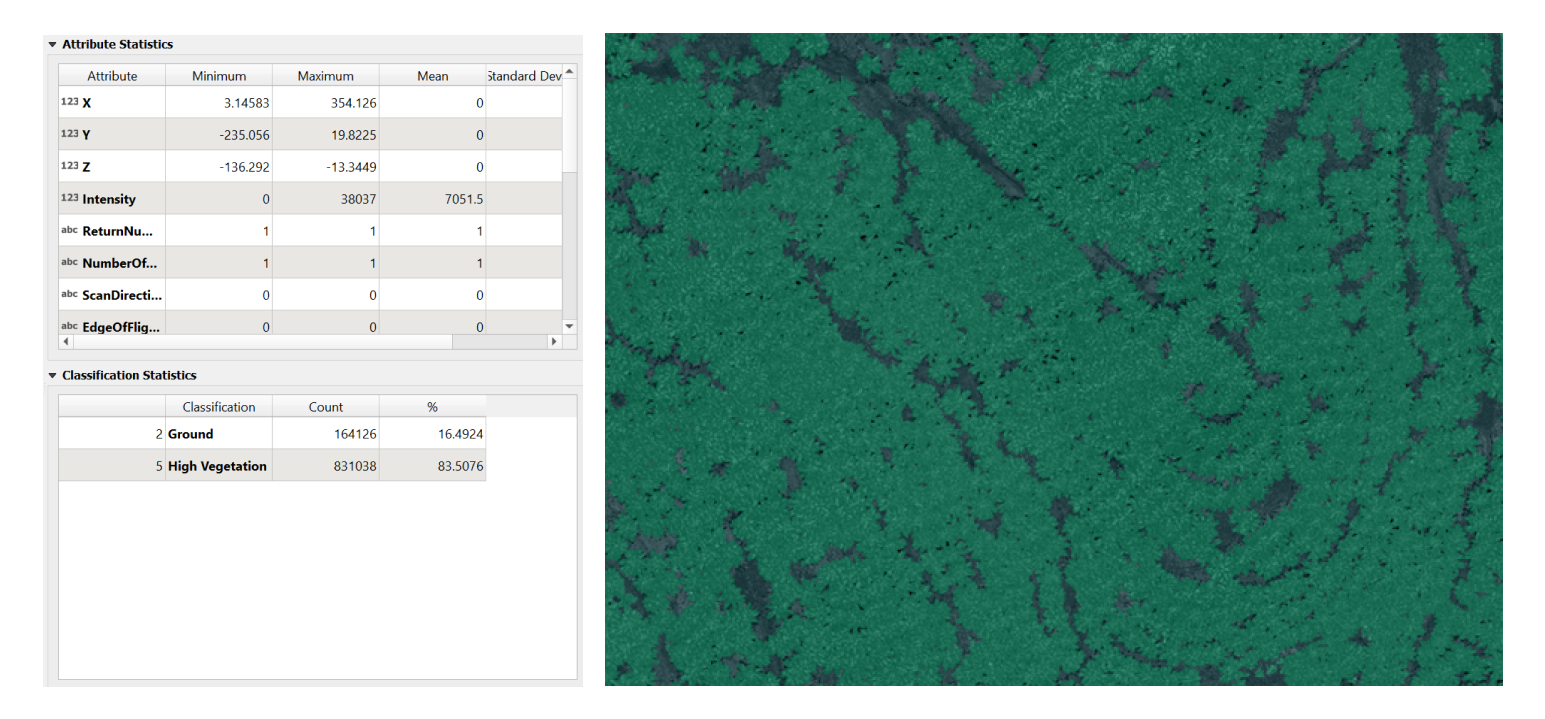
\includegraphics[scale=0.2]{Images/classify.png}
    \caption{Point cloud data which is classified. }
\end{figure}

Lidar is advanced remote sensing technology where it can provide accurate elevation data for both topographic surfaces and above-ground objects \cite{1}. Therefore, every lidar point can have a classification that indicates the different types of objects they reflected. This point classification process is a preprocessor for the derivation of secondary information such as visualizing the data and segmenting individual trees and the classified points will be used for further analysis. 

Our goal is to separate the trees, and we will go through several steps for that goal, but the first step is to separate the ground and ground points. Distinguishing the ground and non-ground points enables the construction of a continuous terrain elevation model such as the Digital Terrain Model (DTM) which will be used in further steps. We are going to use the progressive morphological filter described in \cite{6}. This method will take window size and threshold size as parameters to compare and remove the points based on the threshold and iterate them with a bigger window size. 

The next step is to generate the CHM (Canopy Height model) where we could find out the trees with height information. However, it may cause a problem because the height will be measured on an irregular basis (different shapes and heights of terrain). In other words, non-trees can also be recognized as trees due to the irregular height of the terrain. To reduce the error, we will create the DTM (Digital Terrain Model) by using the classified points above. DTM is a model of the ground surface where all buildings and trees are removed. Using DTM, we can normalize the point cloud of terrain by subtracting the DTM from LAS data. So now, all the elevation in data is relative to the ground surface in which all the points are 0. And this allows comparison of above vegetation heights and the area we collect the data can be minimized. 

With the normalized data, we can generate the CHM (Canopy Height model) which refers to the vertical distance of the branches and leaves of the forest canopy from the ground \cite{7}. And we will use point-to-raster to generate CHM. Point-to-raster is rasterizing the points according to predefined spatial resolution, so it is extremely simple and fast. However, there is one problem with the CHM generated. It contains unnatural black holes also called “pits” that appear in the image which are caused by too high resolution. In this case, the value of the pixel may be undefined since some pixels can be in an area without any points. Therefore, we will smooth the CHM by interpolating the empty pixels.

\begin{figure}[H]
    \centering
    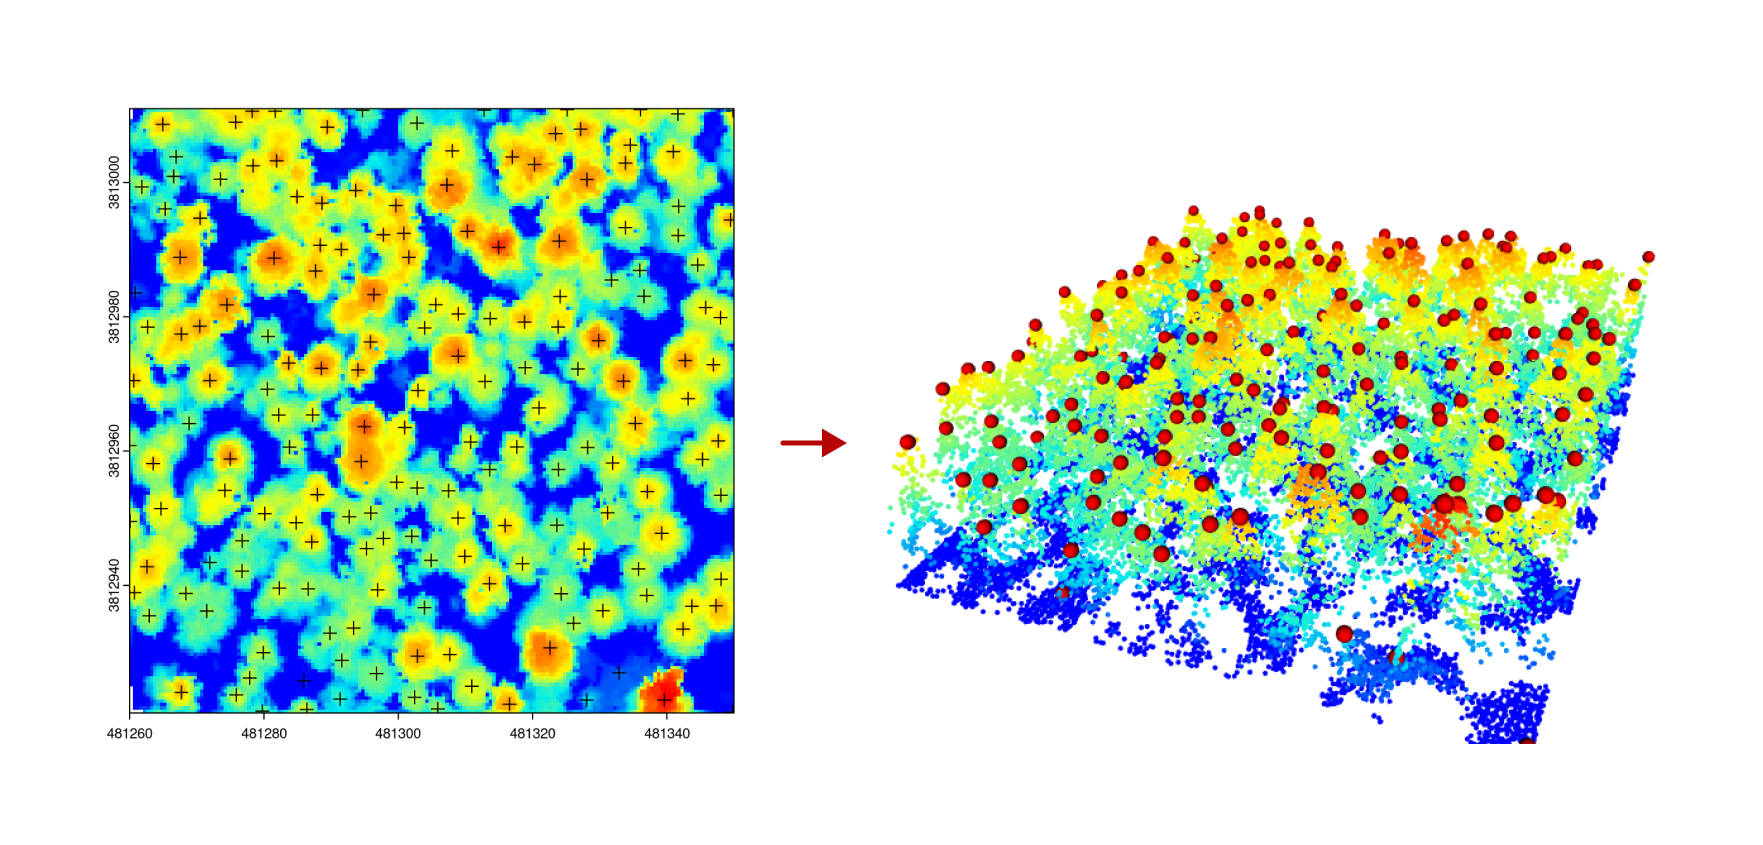
\includegraphics[scale=0.2]{Images/treetop.png}
    \caption{Tree tops detected and visualized with CHM}
\end{figure}

Using the height information in CHM, we will detect the location of individual trees. We will use LMF (Local Maxima Filter) to find treetops. Maxima is extracted with a sliding filter of variable size. Firstly, we will set the size of the window where the algorithm will figure out if the point is the local highest. The size of the window is correlated with the number of trees to be found \cite{8}. If the window is too big, we might miss smaller trees that are hidden by big trees that contain the highest points. Therefore, it is also important to find the most appropriate size for the data. 

\begin{figure}[H]
    \centering
    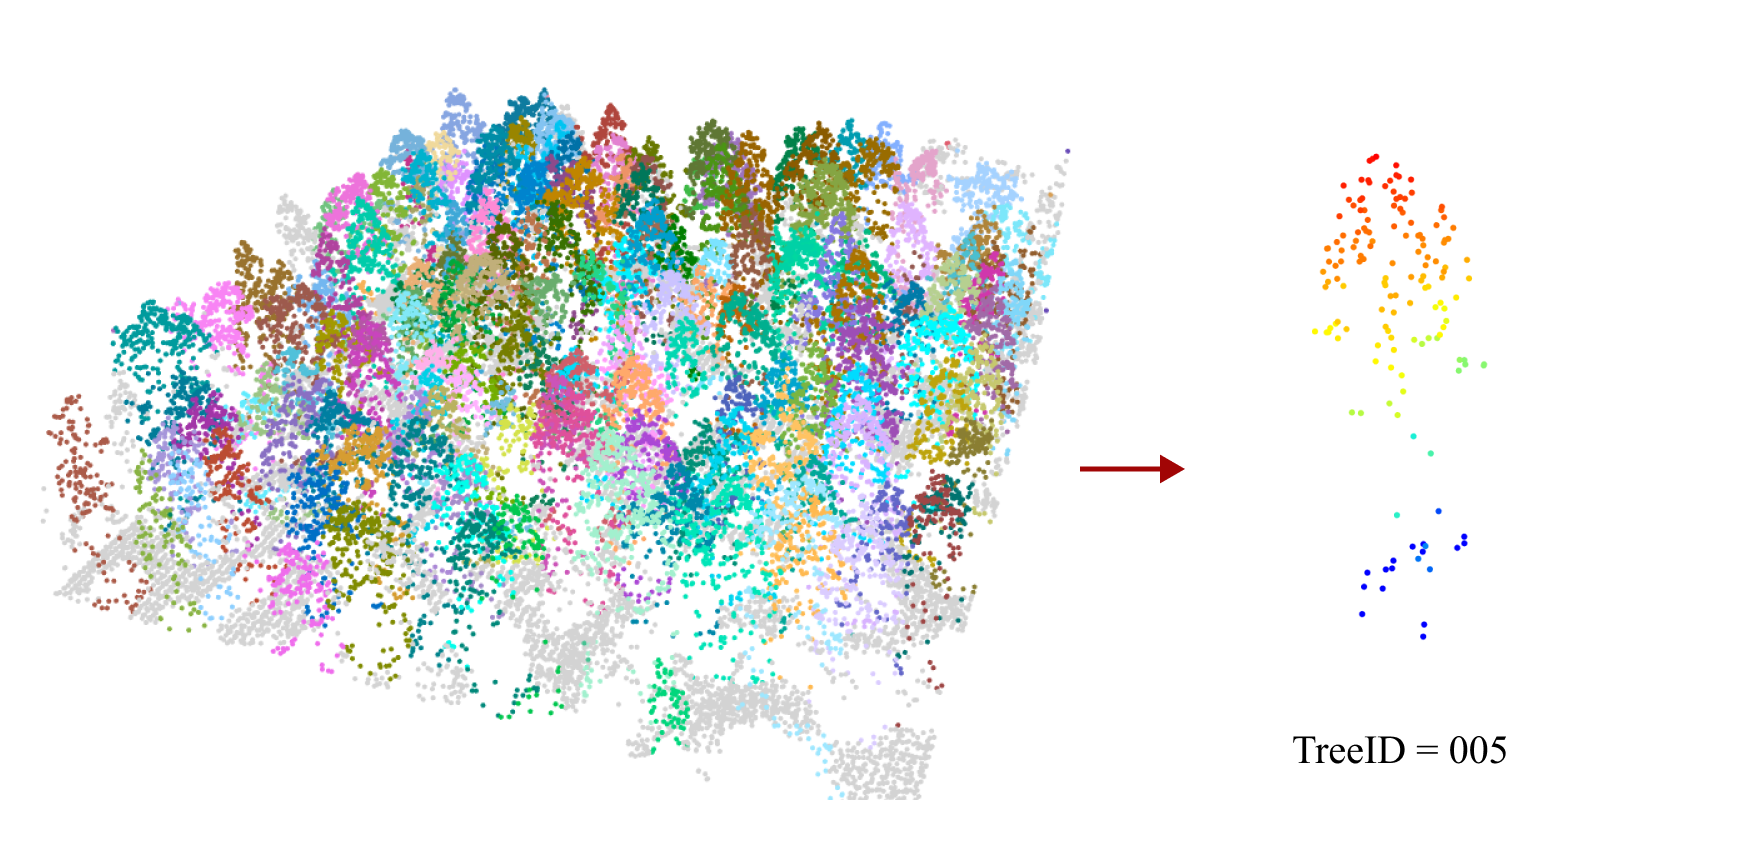
\includegraphics[scale=0.2]{Images/treeseg.png}
    \caption{Unique colour and ID assigned to each individual tree}
\end{figure}

After finding the treetops, we are going to segment individual trees by using the dalponte2016 algorithm. This is a region-growing algorithm developed by Dalpnote and Coomes \cite{9}. It will read the treetops from CHM. And it will take several thresholds set for tree, seeds, and crown as parameters to add pixels based on the treetops we read. For example, if we set the threshold for a tree to 2 and if the height of the pixel is below the threshold, the pixel would not be added. In the case of the crown threshold, if the height of the pixel is greater than the current mean height of the region multiplied by the threshold value, the pixel will be added to the region \cite{10}. At the end of the process, only the pixels that make up the tree will remain.

A huge amount of point data will all represent different trees. However, during tree segmentation, there may be collisions with point data composing other trees. And to prevent this, we will calculate the convex hull of each tree to make it unambiguous. After segmentation, each tree is going to be stored in a file.

\subsection{Requirement Specification}

Functional Requirements:

\begin{itemize}
    \item The system will be able to read the cloud data in a LAS file. \item The system will generate the 3D model of terrain using Lidar data. \item The system will classify the ground and non-ground points. \item The system will normalize the height of the terrain. \item The system will generate a Canopy Height model (CHM). Also, it will be able to smooth the CHM. \item The system will detect the treetops from the terrain using a Local Maxima Filter (LMF). \item The system will segment trees using watershed algorithms. \item The system will assign tree ID to all trees detected. \item The system will be able to segment individual trees according to ID. \item The system will calculate all tree metrics and convex hulls.
\end{itemize}

Non-Functional Requirements:

\begin{itemize}
    \item The system will allow users to analyze the oil palm tree such as measuring the length of the leaves and the height of the tree. \item The system will allow users to zoom in and out of the 3D model of the terrain. \item Also, the system will allow users to turn 360 the 3D model of terrain to view it in every aspect. \item The system will be hosted locally.
\end{itemize}

\subsection{System Design}

The use case diagram of the software:

\begin{figure}[H]
    \centering
    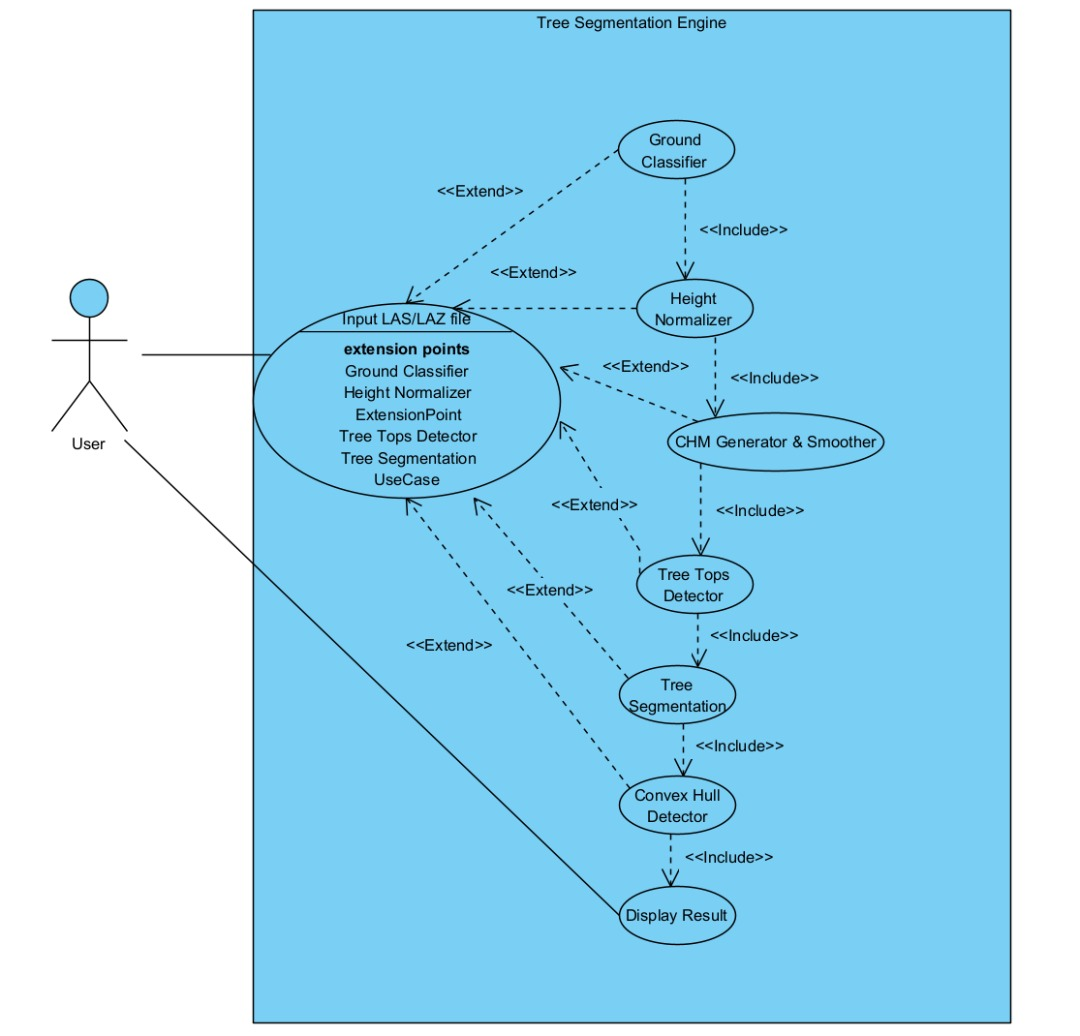
\includegraphics[scale=0.4]{Images/01.jpg}
\end{figure}
\newpage
The sequence diagram of the ground classification process:

\begin{figure}[H]
    \centering
    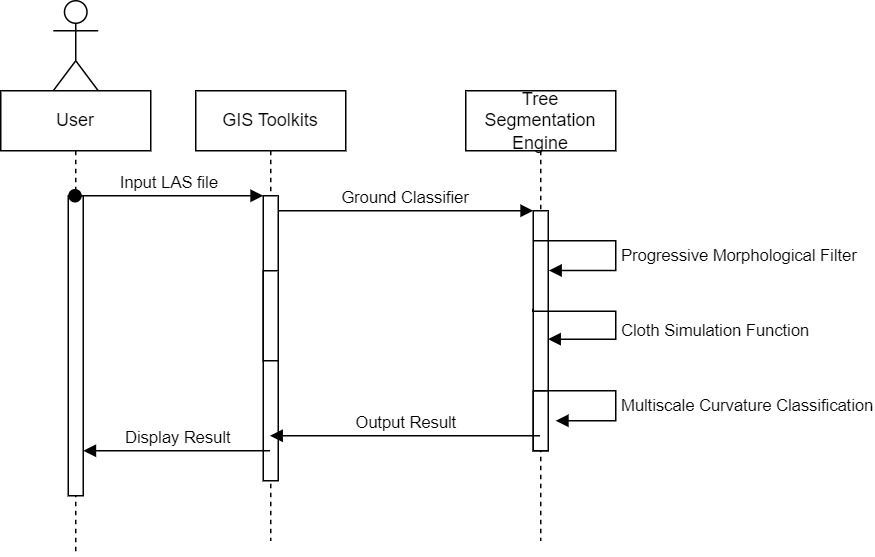
\includegraphics[scale=0.4]{Images/sequenceDiagram-Ground Classifier.jpg}
\end{figure}

The sequence diagram of the height normalization process:

\begin{figure}[H]
    \centering
    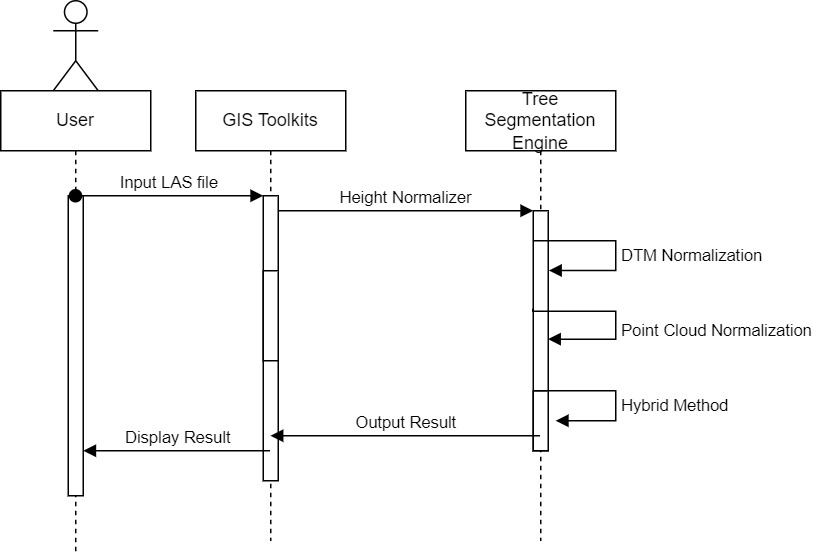
\includegraphics[scale=0.4]{Images/sequenceDiagram-Height Normalizer.jpg}
\end{figure}
\newpage
The sequence diagram of the CHM generating and smoothing process:

\begin{figure}[H]
    \centering
    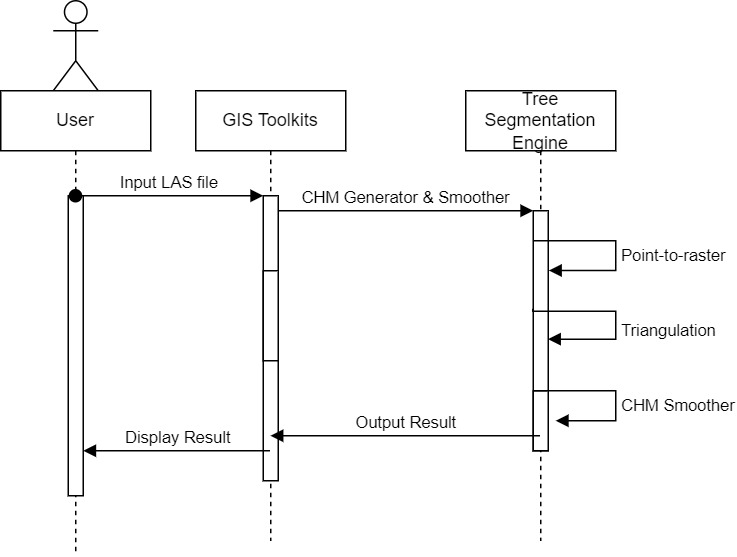
\includegraphics[scale=0.4]{Images/sequenceDiagram-CHM Generator & Smoother.jpg}
\end{figure}

The sequence diagram of the tree tops detection process:

\begin{figure}[H]
    \centering
    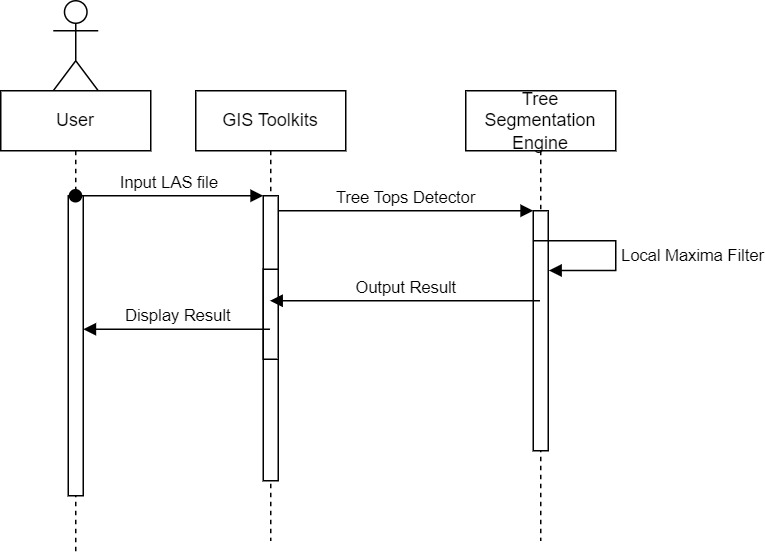
\includegraphics[scale=0.4]{Images/sequenceDiagram-Tree Tops Detector.jpg}
\end{figure}
\newpage
The sequence diagram of the tree segmentation process:

\begin{figure}[H]
    \centering
    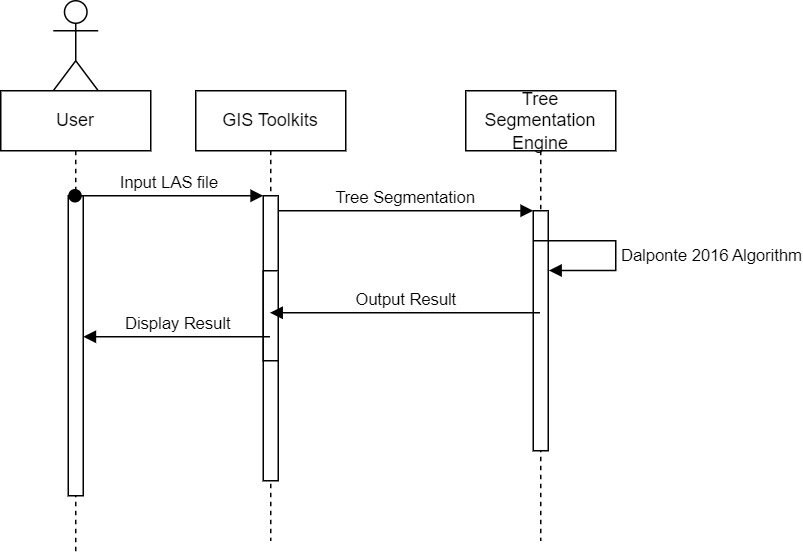
\includegraphics[scale=0.4]{Images/sequenceDiagram-Tree Segmentation.jpg}
\end{figure}

The sequence diagram of the convex hull generating process:

\begin{figure}[H]
    \centering
    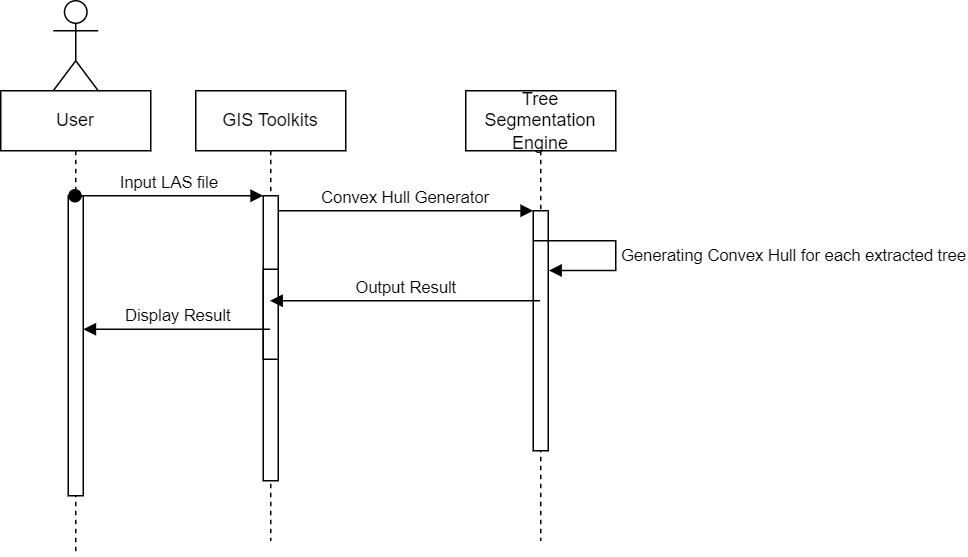
\includegraphics[scale=0.4]{Images/sequenceDiagram-Convex Hull.jpg}
\end{figure}

\section{Technology Stack}

\begin{figure}[H]
    \centering
    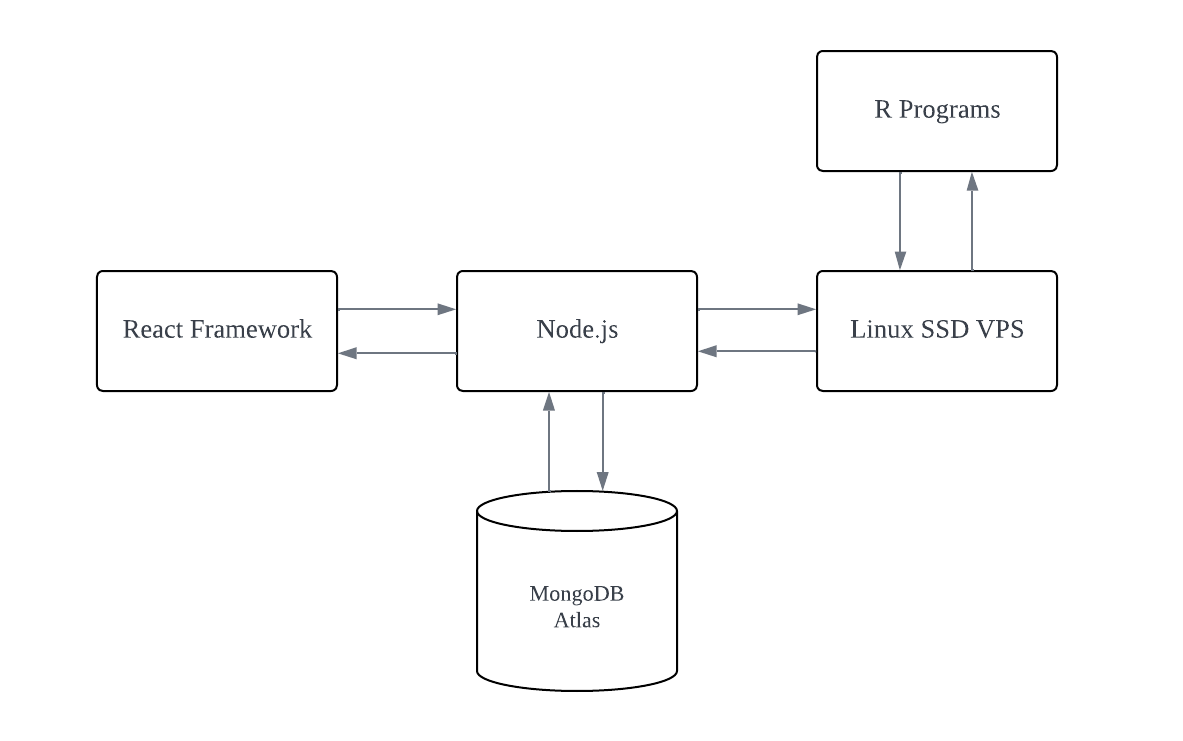
\includegraphics[scale=0.6]{Images/tech.png}
\end{figure}


\subsection{R Language}

The main language used in this project is R. It is a programming language mainly used for statistical analysis, graphical representation, and reporting. Our team chooses to use R because it contains a lot of pre-existing libraries/packages that are convenient for working with LiDAR data. 

\subsection{React}

We choose to use React as our frontend framework, which has a strong ability in creating reusable User Interface components. React is a declarative, efficient, and flexible JavaScript library that helps develop fast and user-friendly web applications.

\subsection{Node.js}

Since we are hosting our software as a web application, we choose to use Node.js to handle the server-side tasks. Node.js is easily employed as a server-side proxy, where it can handle many simultaneous connections in a nonblocking manner.

\subsection{Mongo Database}

MongoDB is a NoSQL database management application. We choose to use Mongo Database Cloud Version (MongoDB Atlas) to connect directly to our web application in order to manage our structured and unstructured data easily.

\subsection{GitHub}

GitHub is used actively throughout the development journey of our team for version control, collaboration, and CI/CD pipeline.

\section{Discussion}

The project given to us is in a relatively unknown field for us university students. Before this project, we had little to no experience in the agricultural industry, but due to the necessity of this project, we were forced to familiarize ourselves with said industry fairly quickly. We made a surprising amount of progress thanks to the methodology chart provided by our client and the plentiful amount of R packages available regarding LAS data. Our client seemed to be satisfied with what we had accomplished so far in the next meeting we had since the first one we had with them.

However, this did not mean that we did not run into any issues. At the time, while we had already discussed and agreed upon separating the different outputs regarding the different stages of the tree segmentation algorithm in a prior meeting, we were not able to implement it and demonstrate it by the second meeting with our client. Our supervisor also requested to see such an implementation which would be a bit more challenging to carry out but it would make the user experience a lot better. This also means more work for the front end but our front end was quite lacking in elements to display so it was welcome to work.

We also had issues with the LAS data provided by the client because there were some incomplete values in the data leading to the program crashing. After all, the algorithms did not have error handling included yet. We were only able to generate images to demonstrate using online publicly available sample LAS data. We agreed that the best way to overcome this issue was by preprocessing the LAS data given by the user to make sure that all the values are valid.

So far our progress is satisfactory but we still have a long way to go in terms of building a final product. The group members, myself included, are still in the process of familiarizing ourselves with the industry as we were unable to grasp how the image produced by the individual tree segmentation algorithm could help serve any useful purpose in any way. To us, it just looks like a mess of dots but to the researchers, it probably makes a lot more sense. Our goal is to help reduce the effort and cost of collecting data for large oil palm plantations and slowly but surely we are coming closer to achieving it.

\section{Prototyping}

\subsection{Low-Fidelity Prototype}

\begin{figure}[H]
    \centering
    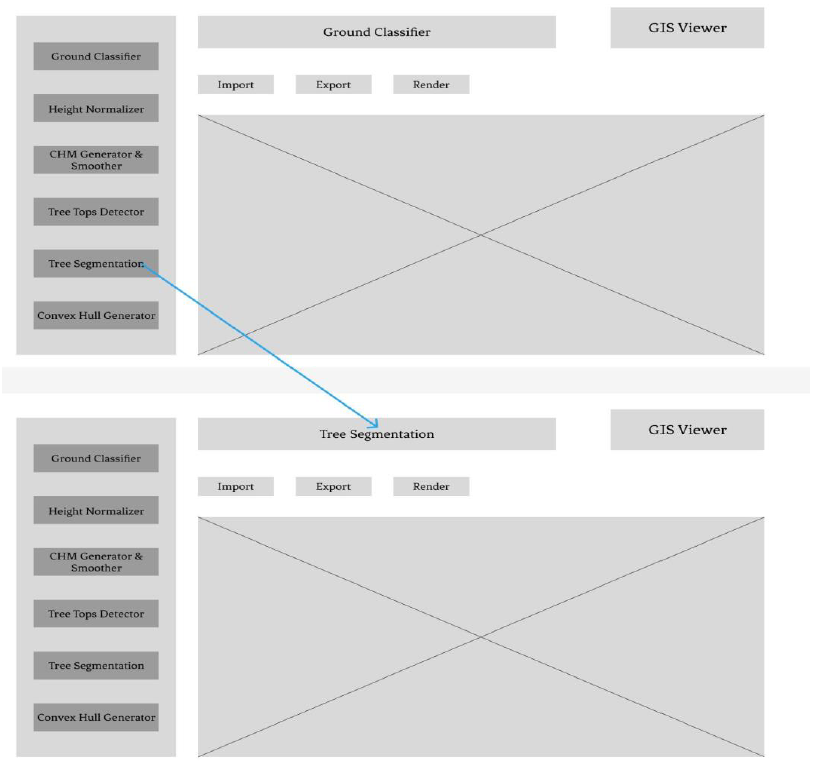
\includegraphics[width=\textwidth]{Images/02.png}
    \caption{Low-Fidelity of the GUI}
    \label{fig:1}
\end{figure}


Figure \ref{fig:1} shows the Guide User Interface (GUI) of the GIS when the user enters the website. In Low-Fidelity Prototype, we make a wireframe on how our GUI should look like and ensure it is simple and user-friendly. When the user clicks on the “Tree Segmentation” button on the left side of the layout, the interface will change from Ground Classifier to Tree Segmentation to perform the specific algorithm that the user clicked. Before performing the algorithm, the user must import the LAS file they want from their local machine to the GUI by clicking the “Import” button and render the LAS file to show the output based on the user's choices on the key features. After the output has been shown, we planned to make an interactable web where users can interact with the output shown by zooming in and out, a 360 viewer on the output data, and able to export the output data by clicking the “Output” button.

\subsection{High-Fidelity Prototype}

\begin{figure}[H]
    \centering
    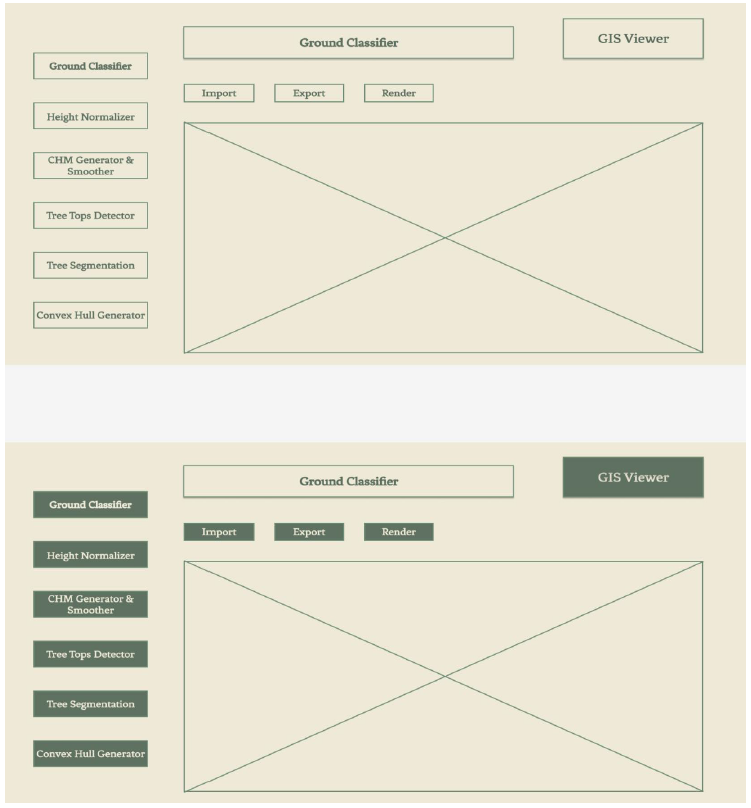
\includegraphics[width=\textwidth]{Images/03.png}
    \caption{Mid-Fidelity of the GUI}
    \label{fig:2}
\end{figure}

Figure \ref{fig:2} shows the GUI has been filled with colors. We choose to have this color theme to fit in our project (GIS) and to ensure that the color theme is simple and easy to read. When the user hovers over the button, it will change the color of the button to bring a better visual effect to the user and also to enhance the GUI’s interactivity.

\subsection{Flowchart}

\begin{figure}[H]
    \centering
    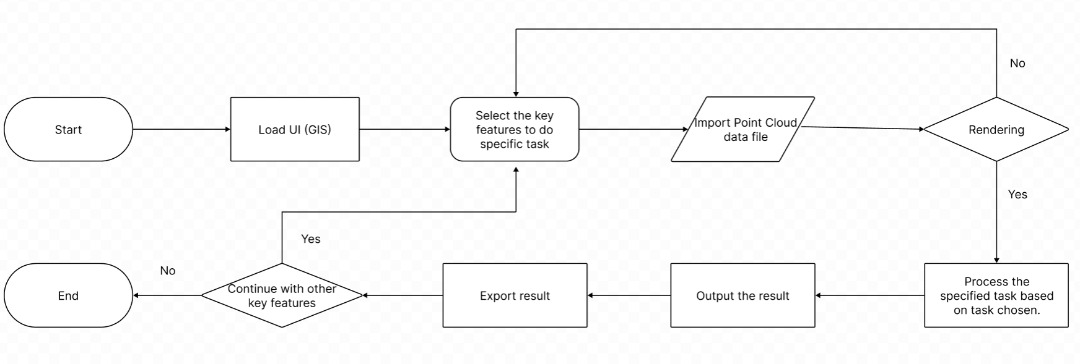
\includegraphics[width=\textwidth]{Images/flow.jpeg}
    \caption{Flowchart of the GUI}
    \label{fig:3}
\end{figure}

When the user enters the website, first the GUI will be loaded, then the user can first select the key features they want to perform the specific task based on the selected key feature. After selecting the key feature, the user must import the LAS file into the GUI and render the file to perform the algorithm based on the selected key features and output the result on the tab. Furthermore, the user can export the output as an image file and still be able to select the other key features to see the respective output.

\section{Time Plan}

\begin{figure}[H]
    \centering
    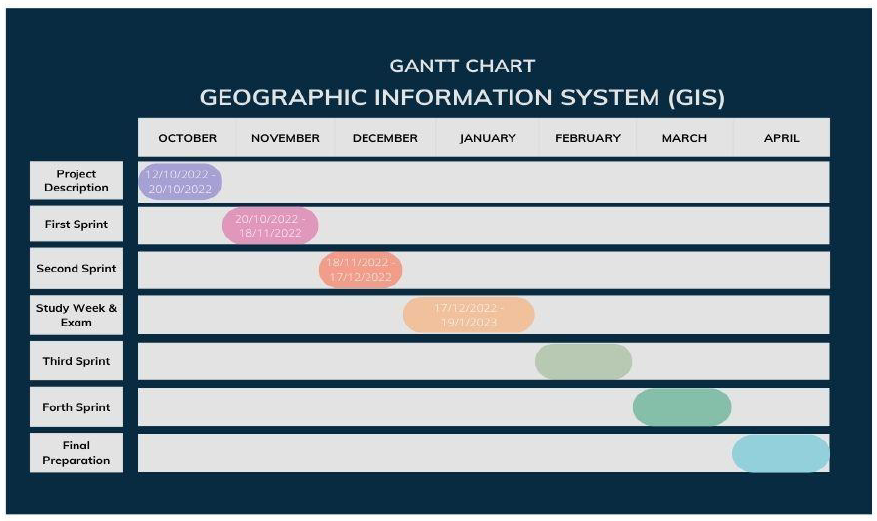
\includegraphics[width=\textwidth]{Images/05.png}
    \caption{Gantt Chart}
    \label{fig:4}
\end{figure}

Mini-Scrum Guide was referenced to assist us in managing our project to plan and discuss our project timeline wisely. In this project, the scrum master is Zhan Choon and his duties are to ensure that the entire team is on the right pace and track, monitor the progression of every teammate, and be able to help and answer teammates’ questions and difficulties to avoid any conflicts between team members. Weekly meetings usually will be held on every Wednesday to discuss the following plans and to solve the issues they are currently facing.

\subsection{Planned Events}

Based on the above figure 4, the first task of the project which was Project Description was discussed among the team members and it required us to sign the ethics form during the period of 12th Oct – 20th Oct. During this period, the team decided to choose R as the main programming language to develop our project as this language provides packages to allow us to implement the key features easier and conveniently. Furthermore, we choose Python as the programming language to develop our front end as Python has an open-source library called “Plotly” that can be used for data visualization. With the help of the Mini-Scrum Guide, the team has decided to hold a meeting once a week to ensure that the tasks assigned to each of the team members have no issues and can follow up so that we can accomplish our main objective which was having 1 prototype before the end of this first semester.


Before meeting with the client, there were many questions in our head as we had no clue what this project is about and what we are going to do in this project. Thus, we do our research and prepare some questions which will be reviewed by our supervisor before meeting with our client. After meeting the client, we have a clearer picture of what are the requirements of the client and what are we going to achieve in this project. We started to discuss the tasks given and distribute the task among the team members. Next, we started coding and using GitHub as our version control to avoid any data loss.

We met with our client, Dr. Chen, and Dr. Iman, our supervisor during the 1\textsuperscript{st} sprint to get some advice on the system requirement and important specifications of this project. The first milestone for the 1\textsuperscript{st} sprint is to complete the requirements that the client requested and build an algorithm that manages to segmentate the vegetation out from the LAS File by the end of this sprint. One of the team members, Zhi Xuan managed to build an algorithm which able to segment the vegetation using the LAS file that was found in online resources. This provides immense progress to our project, and we have more time to focus on designing our front-end layout and creating a GUI. By the end of this 1\textsuperscript{st} sprint, our supervisor and client were reviewing our program and asking us to run the program to do tree segmentation by using the LAS file that was provided by the client but unfortunately, we are unable to do tree segmentation on that but other LAS file samples were fine. We have no clue why the data that was provided by our client is unable to do tree segmentation.

In the 2\textsuperscript{nd} sprint, due to unexpected circumstances, we were delayed in implementing our front end as we were solving why the LAS file provided by our client is not working on our program and trying to look for more solutions online. Fortunately, we were able to find out why it is not working on our program as the LAS file that is provided by our client is fully raw data and all the point cloud data are not classified hence some of the points will be in ‘NULL’ as the program does not recognize what this point was. However, we lack time to complete our original plan due to unforeseen circumstances and hence have to initiate our front-end on the next sprint.

\subsection{Future Event}

During the period of 17\textsuperscript{th} Dec – 19\textsuperscript{th} Jan, we planned to continue working on building a GUI front end to keep our project in progress. During the 3\textsuperscript{rd} sprint, we will continue building the front end and connecting every key feature to the front end which will be reviewed by our client, Dr. Chen. After reviewing from the client, we will start making some minor changes and fixing bugs in the 4\textsuperscript{th} sprint and presenting the app during the open day.

\subsection{Burndown Chart}

\begin{figure}[H]
    \centering
    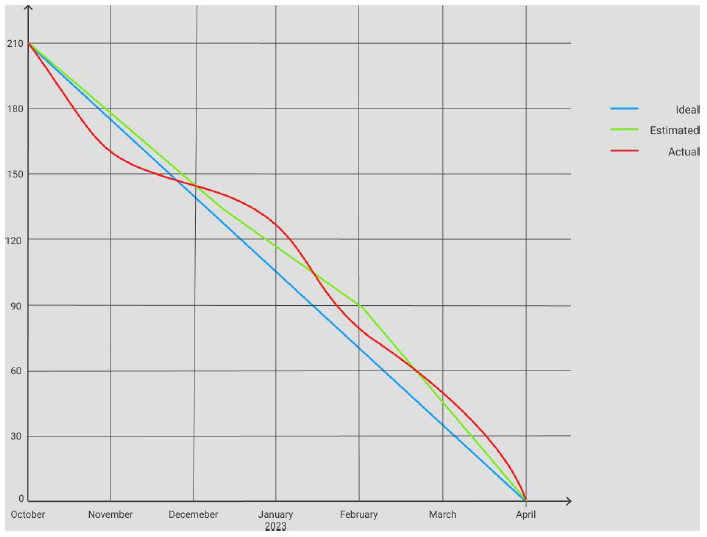
\includegraphics[width=\textwidth]{Images/06.png}
\end{figure}


\section{Conclusion}

The oil palm field has been impacted by the development of the Tree Segmentation Engine as it is one of the key sources of national income and it is crucial to managing the oil palm plantation effectively. With the help of Tree Segmentation Engine, it is more time and resource efficient as users can process the point cloud data and perform tree segmentation tasks to analyze every vegetation compared to the conventional methods such as surveying physically the plantation. Hence, more research and innovations are required to continue developing the Tree Segmentation Engine to increase the work efficiency to allow analysis-related tasks more precise and easier in the future.

\newpage

\bibliographystyle{ieeetr}
\bibliography{refs}

\nocite{*}


\end{document}
